\Opensolutionfile{ans}[ans/ansCD2D1-5-H]
\begin{dang}{Điểm đặc biệt thuộc đồ thị hàm số}.
\end{dang}
\paragraph{Các ví dụ}
\begin{vd}%[2D1Y5-7]%Ví dụ 1.%[Trần Ngọc Phú]
	Cho hàm số $y=x^4-8x^2+1$ có đồ thị $(C)$. Điểm nào sau đây thuộc đồ thị $(C)$? 
	\choice
	{$N(2;-16)$}
	{$B(-1; 8)$}
	{$A(4; 128)$}
	{\True $M(3; 10)$}
	\loigiai{
		Ta có điểm $M(3; 10)$ thuộc đồ thị $(C)$ vì $81-72+1=10$.}
\end{vd}
\begin{vd}%[2D1Y5-2]%Ví dụ 2.%[Trần Ngọc Phú]
	Tìm tất cả các điểm thuộc đồ thị hàm số $y=\dfrac{2x+1}{x-1}$ có khoảng cách đến trục hoành bằng $1$. 
	\choice
	{\True $M(0;-1)$; $N(-2;1)$}
	{$M(-2;1)$}
	{$M(0;-1)$; $N(-1;-1)$}
	{$M(0;-1)$}
	\loigiai{
		Ta có $M\left(x_0;\dfrac{2x_0+1}{x_0-1}\right)$ thuộc đồ thị hàm số.
		\begin{eqnarray*}
	 {d}(M,Ox)=1&\Leftrightarrow&\left|\dfrac{2x_0+1}{x_0-1}\right|=1\\&\Leftrightarrow&\hoac{&2x_0+1=x_0-1\\&2x_0+1=-x_0+1}\\&\Leftrightarrow&\hoac{&x_0=-2&\Rightarrow& N(-2;1)\\&x_0=0&\Rightarrow& M(0;-1).}
		\end{eqnarray*}
		}
\end{vd}
\begin{vd}%[2D1B5-2]%Ví dụ 3.%[Trần Ngọc Phú]
	Biết đồ thị hàm số $y=x^3-3x^2+m$ có điểm uốn nằm trên đường thẳng $y=x$. Tính giá trị của tham số $m$. 
	\choice
	{$m=1$}
	{$m=-1$}
	{\True $m=3$}
	{$m=2$}
	\loigiai{
		$y'=3x^2-6x; y''=6x-6$
		$y''=6x-6=0\Leftrightarrow x=1$.\\
		Suy ra điểm uốn $I(1;m-2)$.\\
		Để điểm uốn nằm trên đường thẳng $y=x\Leftrightarrow m-2=1\Leftrightarrow m=3$.}
\end{vd}
\begin{vd}%[2D1B5-2]%Ví dụ 4.%[Trần Ngọc Phú]
	$A,B$ là hai điểm di động và thuộc hai nhánh khác nhau của đồ thị $y=\dfrac{2x-1}{x+2}$. Khi đó khoảng cách $AB$ bé nhất là
	\choice
	{$2\sqrt{5}$}
	{$\sqrt{10}$}
	{$\sqrt{5}$}
	{\True $2\sqrt{10}$}
	\loigiai{
		Vì $A,B$ thuộc hai nhánh của đồ thị $y=\dfrac{2x-1}{x+2}$\\ nên $A\left(a;2-\dfrac{5}{a+2}\right);B\left(b;2-\dfrac{5}{b+2}\right)$ với $a >-2;b <-2$.\\
		Khi đó $AB^2=(a-b)^2\cdot\left[1+\dfrac{25}{(a+2)^2(b+2)^2}\right]=\left[(a+2)+(-b-2)\right]^2\cdot\left[1+\dfrac{25}{(a+2)^2(-b-2)^2}\right]$.\\
		Áp dụng bất đẳng thức Cô – si ta có:\\
		$\left[(a+2)+(-b-2)\right]^2\geq 4(a+2)(-b-2)$.\\
		$1+\dfrac{25}{(a+2)^2\cdot (-b-2)^2}\geq\dfrac{10}{(a+2)(-b-2)}$.\\
		Từ và suy ra $AB^2\geq 40\Rightarrow AB\geq 2\sqrt{10}$.\\
		Dấu xảy ra khi và chỉ khi $\heva{&a+2=-2-b\\&1=\dfrac{25}{(a+2)^2(-2-b)^2}}\Leftrightarrow\heva{&a=\sqrt{5}-2\\&b=-2-\sqrt{5}.}$ \\
		Vậy $AB_{\min} =2\sqrt{10}$.}
\end{vd}
\paragraph{Câu hỏi trắc nghiệm}
\begin{ex}%[2D1Y5-1]%Câu 1.%[Trần Ngọc Phú]
	Tìm khẳng định \textbf{đúng} trong các khẳng định sau: 
	\choice
	{Đồ thị hàm số bậc ba luôn có trục đối xứng}
	{\True Đồ thị hàm số bậc ba luôn có tâm đối xứng}
	{Trục đối xứng của đồ thị hàm số bậc ba là đường thẳng nối hai điểm cực trị của đồ thị hàm số bậc ba đó}
	{Đồ thi hàm số bậc ba luôn nhận gốc tọa độ làm tâm đối xứng}
	\loigiai{
		Đồ thị hàm số bậc ba luôn có tâm đối xứng với tâm đối xứng là một điểm thuộc đồ thi hàm số có hoành độ là nghiệm của phương trình $y''=0$.}
\end{ex}
\begin{ex}%[2D1Y5-2]%Câu 2.%[Trần Ngọc Phú]
	Đồ thị của hàm số nào sau đây \textbf{không} đi qua điểm $M(1;-2)$?
	\choice
	{$y=\dfrac{3x-1}{x-2}$}
	{$y=x^3-3x$}
	{\True $y=-x^3+3x-1$}
	{$y=x^4-x^2-2$}
	\loigiai{
		Xét hàm số $y=-x^3+3x-1$.\\
		Với $x=1\Rightarrow y=1$.\\ Vậy đồ thị hàm số $y=-x^3+3x-1$ \textbf{không} đi qua điểm $M(1;-2)$.}
\end{ex}
\begin{ex}%[2D1Y5-2]%Câu 3.%[Trần Ngọc Phú]
	Cho hàm số $y=x^4-x^2+1$ có đồ thị $(C)$. Điểm nào sau đây thuộc đồ thị $(C)$?
	\choice
	{$A(1;0)$}
	{\True $B(2;13)$}
	{$C(-1;3)$}
	{$D(-2;-13)$}
	\loigiai{Ta có $13=2^4-2^2+1$. Do đó điểm $B$ thuộc đồ thị hàm số $\left(C \right)$ }
\end{ex}
\begin{ex}%[2D1Y5-2]%Câu 4.%[Trần Ngọc Phú]
	Cho hàm số $y=x^4-3x^2-5$ có đồ thị $(C)$. Điểm nào sau đây thuộc đồ thị $(C)$?
	\choice
	{$A(1;3)$}
	{\True $B(2;-1)$}
	{$C(-1;-3)$}
	{$(-2;-9)$}
	\loigiai{
		Ta có: $2^4-3\cdot 2^2-5=-1$ nên $B\in(C)$.}
\end{ex}
\begin{ex}%[2D1Y5-2]%Câu 5.%[Trần Ngọc Phú]
	\immini
	{Cho hàm số $y=f(x)$ có đồ thị như hình bên. 
	Các khẳng định sau:\\
	$(I)\lim\limits_{x\to 1^-} f(x)=-\infty$\\
	$(II)\lim\limits_{x\to-2^+} f(x)=-\infty$\\
	$(III)\lim\limits_{x\to+\infty} f(x)=-\infty$.\\
	$(IV)\lim\limits_{x\to-2^-} f(x)=+\infty$.\\
	Số khẳng định đúng là 
	\choice
	{$4$}
	{\True $3$}
	{$1$}
	{$2$}
}
{\begin{tikzpicture}[scale=0.7,font=\footnotesize,line join = round, line cap = round,>=stealth]
	\def\hsf{(-2*(\x)-5)/((\x)+2)}
	\def\hsg{(4*(\x)-3)/(4*(\x)-4)}
	\def\hsh{(-1*(\x)^3+2)/((\x)^2+(\x)-2)}
	\draw[->] (-5,0)--(0,0)node[below left]{$O$}--(6,0)node[below]{$x$};
	\draw[->] (0,-4.5)--(0,5)node[left]{$y$};
	\draw[] (-5,1)--(6,1) (-2,-4.5)--(-2,5) (1,-4.5)--(1,5) (-5,-2)--(6,-2);
	\draw[samples=100,domain=-5:-2.15,smooth] plot (\x, {\hsf});
	\draw[samples=100,domain=1.1:5,smooth] plot (\x, {\hsg});
	\draw[samples=100,domain=-1.5:0.85,smooth] plot (\x, {\hsh});
	\fill (0,-2)node[below left]{$-2$} circle (1.5pt);\fill (0,1) node[above left]{$1$} circle (1.5pt);\fill (-2,0)node[above right]{$-2$} circle (1.5pt);\fill (1,0) node[above left]{$1$} circle (1.5pt);\fill (0,-1) node[right]{$-1$} circle (1.5pt);
	\end{tikzpicture}	
}
	\loigiai{$(I)\lim\limits_{x\to 1^-} f(x)=-\infty$. (\textbf{đúng})\\
		$(II)\lim\limits_{x\to-2^+} f(x)=-\infty$. (\textbf{đúng})\\
		$(III)\lim\limits_{x\to+\infty} f(x)=-\infty$ (\textbf{sai}) vì $\lim\limits_{x\to+\infty} f(x)=1$.\\
		$(IV)\lim\limits_{x\to-2^-} f(x)=+\infty$. (\textbf{đúng})\\
	Vậy số khẳng định đúng là $3$.
	}
\end{ex}
\begin{ex}%[2D1B5-2]%Câu 6.%[Trần Ngọc Phú]
	Cho đồ thị $(C)$ của hàm số: $y=(1-x)(x+2)^2$. Trong các mệnh đề sau, tìm mệnh đề \textbf{sai}: 
	\choice
	{$(C)$ có 2 điểm cực trị}
	{$(C)$ có một điểm uốn}
	{$(C)$ có một tâm đối xứng}
	{\True $(C)$ có một trục đối xứng}
	\loigiai{
		Vì $y=(1-x)(x+2)^2$ là hàm bậc ba nên đồ thị $(C)$ của hàm số không có trục đối xứng.}
\end{ex}
\begin{ex}%[2D1B5-2]%Câu 7.%[Trần Ngọc Phú]
	Khoảng cách từ điểm cực đại của đồ thì hàm số $y=x^3-2x^2+x-1$ đến trục hoành là
	\choice
	{\True $\dfrac{23}{27}$}
	{$\dfrac{1}{9}$}
	{$\dfrac{1}{3}$}
	{$1$}
	\loigiai{
		$y'=3x^2-4x+1$.\\
		$y'=0\Leftrightarrow\hoac{&x=1\\&x=\dfrac{1}{3}}.$\\
		Bảng biến thiên
		\begin{center}
			
\begin{tikzpicture}
			\tkzTabInit[nocadre=false,lgt=1.2,espcl=2.5,deltacl=0.6]
			{$x$/.7,$y'$/.7,$y$/2}
			{$-\infty$ , $\frac{1}{3}$ , $1$ , $+\infty$}
			\tkzTabLine{ ,  + , $0$ , - , $0$ , + , }
			\tkzTabVar{-/$-\infty$ , +/$-\dfrac{23}{27}$, -/$-1$ , +/$+\infty$}
			\end{tikzpicture}
		\end{center}
		Vậy $A\left(\dfrac{1}{3};-\dfrac{23}{27}\right)$ là điểm cực đại của đồ thị hàm số nên $\mathrm{d}(A;x'Ox)=\dfrac{\left|-\dfrac{23}{27}\right|}{\sqrt{1^2}}=\dfrac{23}{27}$.}
\end{ex}
\begin{ex}%[2D1B5-2]%Câu 8.%[Trần Ngọc Phú]
	Tính tổng hoành độ các điểm thuộc đồ thị hàm số $y=x^3-3x^2+2$ cách đều hai điểm $A(12; 1)$ và $B(-6; 3)$. 
	\choice
	{$4$}
	{$-6$}
	{\True $0$}
	{$2$}
	\loigiai{
		Ta có $\overrightarrow{AB}=(-18;2)$ và $I(3;2)$ là trung điểm của $AB$.\\
		Đường trung trực của $AB$ có phương trình: $9x-y-25=0$ hay $y=9x-25$.\\ Hoành độ các điểm thỏa mãn yêu cầu đề bài là nghiệm của phương trình
		\begin{eqnarray*}
		9x-25=x^3-3x^2+2&\Leftrightarrow& x^3-3x^2-9x+27=0\\&\Leftrightarrow&\hoac{&x=3\\&x=-3.}
		\end{eqnarray*}
		  Vậy tổng các hoành độ là $0$.}
\end{ex}
\begin{ex}%[2D1Y5-2]%Câu 9.%[Trần Ngọc Phú]
	Có bao nhiêu điểm thuộc đồ thị hàm số $y=\dfrac{x^2-3x}{x-1}$ có tọa độ nguyên?
	\choice
	{Không có điểm nào}
	{\True $4$ điểm}
	{$2$ điểm}
	{Vô số điểm}
	\loigiai{
		Ta có $y=\dfrac{x^2-3x}{x-1}=x-2-\dfrac{2}{x-1}$.\\
		Do $y\in\mathbb{Z}\Rightarrow\dfrac{2}{x-1}\in\mathbb{Z}\Rightarrow x-1\in\{-2;-1;1;2\}$.\\
		Suy ra $\hoac{&x=-1\\&x=0\\&x=2\\&x=3}\Rightarrow\hoac{&y=-2\\&y=0\\&y=-2\\&y=0}$. Vậy ta có $4$ điểm.}
\end{ex}
\begin{ex}%[2D1Y5-2]%Câu 10.%[Trần Ngọc Phú]
	Số điểm trên đồ thị hàm số $y=\dfrac{2x-1}{x+2}$ có hoành độ và tung độ đều là các số nguyên là 
	\choice
	{\True $4$}
	{$6$}
	{$2$}
	{$3$}
	\loigiai{
		TXĐ $\mathscr{D}=\mathbb{R}\setminus\{-2\}$.\\
		Ta có $y=\dfrac{2(x+2)-5}{x+2} =2-\dfrac{5}{x+2}$.\\
		Có $x, y\in\mathbb{Z}\Leftrightarrow(x+2)\in Ư(5)=\{\pm 1;\pm 5\}$. Vậy có $4$ điểm thỏa mãn yêu cầu bài toán.}
\end{ex}
\begin{ex}%[2D1B5-2]%Câu 11.%[Trần Ngọc Phú]
	Số điểm cố định của đồ thị hàm số $y=x^3+(m-3)x^2-(2m-1)x-3m-3$ là
	\choice
	{\True $2$}
	{$1$}
	{$4$}
	{$3$}
	\loigiai{
		Gọi $M(x;y)$ là điểm cố định của đồ thị hàm số.\\
		Khi đó ta có $y=x^3+(m-3)x^2-(2m-1)x-3m-3$ hay $-x^3+3x^2-x+y+3+m\left(2x-x^2\right)=0$ với mọi giá trị $m$. \\Suy ra $\heva{&2x-x^2=0\\&-x^3+3x^2-x+y+3=0}\Leftrightarrow\heva{&\hoac{&x=0\\&x=2}\\&y=x^3-3x^2+x-3}\Leftrightarrow\hoac{&\heva{&x=0\\&y=-3}\\&\heva{&x=2\\&y=-5.}}$ \\
		Vậy đồ thị hàm số có hai điểm cố định.}
\end{ex}
\begin{ex}%[2D1Y5-6]%Câu 12.%[Trần Ngọc Phú]
	Hình bên là đồ thị của hàm $y=f(x)$. Biết rằng tại các điểm $A, B, C$ đồ thị hàm số có tiếp tuyến được thể hiện như hình vẽ. mệnh đề nào dưới đây đúng?
	\begin{center}
		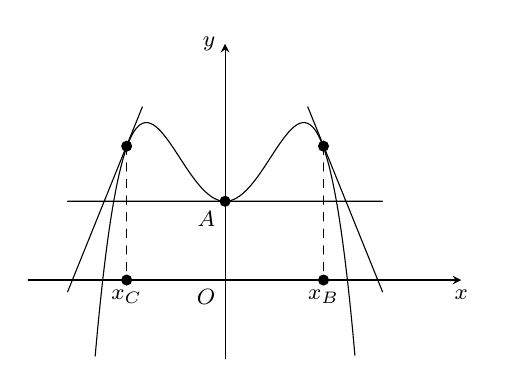
\begin{tikzpicture}[scale=1,font=\footnotesize,line join = round, line cap = round,>=stealth]
		\def\hsf{-1*(\x)^4+2*(\x)^2+1}
		\draw[->] (-2.5,0)--(0,0)node[below left]{$O$}--(3,0)node[below]{$x$};
		\draw[->] (0,-1)--(0,3)node[left]{$y$};
		\draw[dashed,thin] (-1.25,1.7)--(-1.25,0) (1.25,1.7)--(1.25,0);
		\draw[] (-2,-.15)--(-1.05,2.2) (2,-.15)--(1.05,2.2) (-2,1)--(2,1);
		\draw[samples=100,domain=-1.65:1.65,smooth] plot (\x, {\hsf});
		\fill (0,1)node[below left]{$A$} circle (2pt);\fill (-1.25,1.7)circle (2pt);\fill (1.25,1.7)circle (2pt);\fill (-1.25,0)node[below]{$x_C$}circle (2pt);\fill (1.25,0)node[below]{$x_B$}circle (2pt);%\fill (2,0)node[ above right]{$2$} circle (1pt);\fill (1,0)node[below left]{$1$}circle (1pt);\fill (-1,0)node[below left]{$-1$} circle (1.5pt);
		\end{tikzpicture}
	\end{center}
	\choice
	{$f'(x_C)<f'(x_A)<f'(x_B)$}
	{\True $f'(x_B)<f'(x_A)<f'(x_C)$}
	{$f'(x_A)<f'(x_B)<f'(x_C)$}
	{$f'(x_A)<f'(x_C)<f'(x_B)$}
	\loigiai{
		Ta có $f'(x_A)=0$, $f'(x_C)>0$, $f'(x_B)<0$ nên $f'(x_B)<f'(x_A)<f'(x_C)$.}
\end{ex}
\begin{ex}%[2D1B5-2]%Câu 13.%[Trần Ngọc Phú]
	Điểm thuộc đường thẳng $d\colon x-y-1=0$ cách đều hai điểm cực trị của đồ thị hàm số $y=x^3-3x^2+2$ là 
	\choice
	{\True $(1;0)$}
	{$(2;1)$}
	{$(-1;2)$}
	{$(0;-1)$}
	\loigiai{
		Ta có $y'=3x^2-6x$.\\
		$y'=0\Leftrightarrow\hoac{&x=0\\&x=2.}$ \\
		Hai điểm cực trị của hàm số: $A(0;2)$ và $B(2;-2)$.\\
		Điểm thuộc đường thẳng $d\colon x-y-1=0$ là $M(t;t-1)$.
		\begin{eqnarray*}
		M(t;t-1)\,  \text{cách đều hai điểm cực trị của đồ thị hàm số} &\Leftrightarrow& MA=MB \\
		 &\Leftrightarrow& t^2+(t-3)^2=(t-2)^2+(t+1)^2\\&\Leftrightarrow& t=1.
		\end{eqnarray*}
		Vậy $M(1;0)$.}
\end{ex}
\begin{ex}%[2D1B5-2]%Câu 14.%[Trần Ngọc Phú]
	Tìm tất cả các giá trị của tham số m để đồ thị hàm số $y=x^3-3mx^2+3\left(m^2-1\right)x+1-m^2$ có hai điểm phân biệt đối xứng nhau qua gốc tọa độ O. 
	\choice
	{$0<m<1$}
	{$0\leq m<1$ hoặc $m\leq-1$}
	{$m <-1$}
	{\True $0<m<1$ hoặc $m <-1$}
	\loigiai{
		Giả sử $A'$ là điểm đối xứng của $A$ qua $O$ suy ra $ A\left(x_0;y_0 \right)\in \left(C \right)\Rightarrow A'\left(-x_0;-y_0 \right)\in \left(C \right)   $\\
		Khi đó hệ phương trình sau nghiệm\\
		$\begin{aligned}&\heva{&y_0=x_0^3-3mx_0^2+3\left(m^2-1\right)x_0+1-m^2\\&-y_0=-x_0^3-3mx_0^2-3\left(m^2-1\right)x_0+1-m^2}\\&\Rightarrow-6mx^2_0=2-m^2\Rightarrow x^2_0=\dfrac{2-m^2}{-6m}>0\left( m\neq 0\right) \Leftrightarrow 0<m<1\,  \text{hoặc}\, m <-1.\end{aligned}$}
\end{ex}
\begin{ex}%[2D1Y5-1]%Câu 15.%[Trần Ngọc Phú]
	Cho hàm số $y=\dfrac{-4}{3}x^3+8x^2+1$. Mệnh đề nào sau đây đúng?
	\choice
	{\True Điểm cực tiểu của đồ thị hàm số là $C\left( 0;1\right) $}
	{Điểm cực tiểu của hàm số là $B\left( 4;\dfrac{131}{3}\right) $}
	{Điểm cực đại của hàm số là $B\left( 4;\dfrac{131}{3}\right) $}
	{Điểm cực đại của đồ thị hàm số là $C\left( 0;1\right) $}
	\loigiai{
		$y'=-4x^2+16x$.\\
		$y'=0\Leftrightarrow\hoac{&x=0\\&x=4.}$ \\
		Bảng biến thiên
		\begin{center}
			
\begin{tikzpicture}
			\tkzTabInit[nocadre=false,lgt=1.2,espcl=2.5,deltacl=0.6]
			{$x$/.7,$f'(x)$/.7,$f(x)$/2}
			{$-\infty$ , $0$ , $4$ , $+\infty$}
			\tkzTabLine{ ,  - , $0$ , + , $0$ , - , }
			\tkzTabVar{+/$+\infty$ , -/$1$, +/$\dfrac{131}{3}$ , -/$-\infty$}
			\end{tikzpicture}
		\end{center}
	Vậy điểm cực tiểu của đồ thị hàm số là $C\left( 0;1\right) $
	}
\end{ex}
\begin{ex}%[2D1K5-2]%Câu 16.%[Trần Ngọc Phú]
	Biết $A(x_A; y_A)$, $B(x_B; y_B)$ là hai điểm thuộc hai nhánh khác nhau của đồ thị hàm số $y=\dfrac{x+4}{x+1}$ sao cho độ dài đoạn thẳng $AB$ nhỏ nhất. Tính $P=y_A^2+y_B^2-x_Ax_B$. 
	\choice
	{\True $P=10$}
	{$P=6$}
	{$P=6-2\sqrt{3}$}
	{$P=10-\sqrt{3}$}
	\loigiai{
		Ta có $y=\dfrac{x+4}{x+1}=1+\dfrac{3}{x+1}$.\\
		Vì $A, B$ thuộc hai nhánh của đồ thị nên $A\left(x_A; 1+\dfrac{3}{x_A+1}\right), B\left(x_B; 1+\dfrac{3}{x_B+1}\right)$ với $x_A <-1<x_B$.\\
		Đặt $\heva{&x_A=-1-a\\&x_B=-1+b}$ với $a>0, b>0$. Khi đó $\heva{&y_A=1-\dfrac{3}{a}\\&y_B=1+\dfrac{3}{b}.}$ \\
		Ta có $AB^2=(a+b)^2+\left(\dfrac{3}{a}+\dfrac{3}{b}\right)^2=(a+b)^2\left(1+\dfrac{9}{a^2b^2}\right)$.\\
		Áp dụng bất đẳng thức Cô-si ta có: $\heva{&(a+b)^2\geq 4ab\\&1+\dfrac{9}{a^2b^2}\geq\dfrac{6}{ab}.}$ \\
		Từ đó suy ra $AB^2\geq 4ab\times\dfrac{6}{ab}=24$. Do đó $AB$ ngắn nhất bằng $2\sqrt{6}$.\\
		Dấu $=$ xảy ra khi $\heva{&a=b\\&1=\dfrac{9}{a^2b^2}}\Rightarrow a=b=\sqrt{3}\Rightarrow\heva{&A\left(-1-\sqrt{3}; 1-\sqrt{3}\right)\\&B\left(-1+\sqrt{3}; 1+\sqrt{3}\right).}$ \\
		Suy ra $P=y_A^2+y_B^2-x_Ax_B=(1-\sqrt{3})^2+(1+\sqrt{3})^2-\left(-1-\sqrt{3}\right)\left(-1+\sqrt{3}\right)=10$.}
\end{ex}
\begin{ex}%[2D1B5-2]%Câu 17.%[Trần Ngọc Phú]
	Cho hàm số $y=\dfrac{x+2}{x+1}$ có đồ thị $(C)$. Có bao nhiêu điểm thuộc đồ thị $(C)$ mà hoành độ và tung độ đều là các số nguyên?
	\choice
	{$1$}
	{\True $2$}
	{$3$}
	{$4$}
	\loigiai{
		Ta có $y=\dfrac{x+2}{x+1}=1+\dfrac{1}{x+1}$.\\
		Để tọa độ nguyên thì 1 chia hết cho $x+1$ khi đó ta có $\hoac{&x+1=1\\&x+1=-1}\Leftrightarrow\hoac{&x=0\\&x=-2.}$ \\
		Vậy có 2 điểm thuộc $(C)$ thỏa yêu cầu bài toán là $A(0;2), B(-2;0)$.}
\end{ex}
\begin{ex}%[2D1B5-2]%Câu 18.%[Trần Ngọc Phú]
	Cho hàm số $y=x^3-2x+1$. Tìm tất cả các điểm $M$ thuộc đồ thị hàm số sao cho khoảng cách từ $M$ đến trục tung bằng $1$. 
	\choice
	{$M(2;-1)$}
	{$M(1;0)$}
	{\True $M(1;0)$ hoặc $M(-1;2)$}
	{$M(0;1)$ hoặc $M(2;-1)$}
	\loigiai{
		Gọi $M(x_0;y_0)$ nằm trên đồ thị hàm số.\\
		Ta có $d[M,Oy]=|x_0|=1\Leftrightarrow\hoac{&x_0=1\Rightarrow y_0=0\\&x_0=-1\Rightarrow y_0=2.}$ \\
		Vậy $M(1;0)$ và $M(-1;2)$.}
\end{ex}
\begin{ex}%[2D1K5-2]%Câu 19.%[Trần Ngọc Phú]
	Cho hàm số $y=\dfrac{2x}{x-2}$ có đồ thị $(C)$. Tìm giá trị nhỏ nhất $h$ của tổng khoảng cách từ điểm $M$ thuộc $(C)$ tới hai đường thẳng $\Delta_1\colon x-1=0$ và $\Delta_2\colon y-2=0$. 
	\choice
	{$h=2$}
	{\True $h=3$}
	{$h=5$}
	{$h=4$}
	\loigiai{
		TXĐ $\mathscr{D}=\mathbb{R}\setminus\{2\}$.\\
		Gọi $M\left(x_o;\dfrac{2x_o}{x_o-2}\right)\in(C)$.\\
		Ta có $h=\mathrm{d}\left(M,{\Delta}_1\right)+\mathrm{d}\left(M,{\Delta}_2\right)=|x_o-1|+\left|\dfrac{2x_o}{x_o-2}-2\right|=|x_o-1|+\left|\dfrac{4}{x_o-2}\right|$.\\
		+ Với $x_0<1$ thì $h=1-x_0+\dfrac{4}{2-x_0}=2-x_0+\dfrac{4}{2-x_0}-1\geq 2\cdot\sqrt{(2-x_0\cdot)\dfrac{4}{2-x_0}}-1=3$.\\
		Dấu xảy ra khi và chỉ khi $2-x_0=\dfrac{4}{2-x_0}\Leftrightarrow\hoac{&x_0=0\in(-\infty;1)\\&x_0=4\notin(-\infty;1)}\Leftrightarrow x_0=0$.\\
		+ Với $1\leq x_0<2$ thì $h=x_0-1+\dfrac{4}{2-x_0}$.\\
		Ta có $h'=1+\dfrac{4}{(2-x_0)^2}>0,\forall x_0\in[1;2)$.\\
		Hàm số liên tục và đồng biến trên $[1;2)$ nên $h_{\min}=h(1)=4$.\\
		+ Với $x_0>2$ thì $h=x_0-1+\dfrac{4}{x_0-2}=x_0-2+\dfrac{4}{x_0-2}+1\geq 2\cdot\sqrt{(x_0-2)\dfrac{4}{x_0-2}}+1=5$.\\
		Dấu xảy ra khi và chỉ khi $x_0-2=\dfrac{4}{x_0-2}\Leftrightarrow\hoac{&x_0=0\notin(2;+\infty)\\&x_0=4\in(2;+\infty)}\Leftrightarrow x_0=4$.\\
		Vậy $h=3$.\\
		Ta có thể chia trường hợp rồi khảo sát hàm số để tìm GTLN, GTNN hoặc dùng máy tính casio với chức năng table tìm được giá trị nhỏ nhất h của tổng khoảng cách từ điểm M thuộc tới hai đường thẳng đã cho là 3 khi $x_o=0$.\\
		Cách 2: Ta có $h=\mathrm{d}\left(M,{\Delta}_1\right)+\mathrm{d}\left(M,{\Delta}_2\right)=|x_0-1|+\left|\dfrac{2x_0}{x_0-2}-2\right|=|x_0-1|+\left|\dfrac{4}{x_0-2}\right|$.\\
		$=|x_0-2+1|+\dfrac{4}{|x_0-2|}\geq|x_0-2|-1+\dfrac{4}{|x_0-2|}\geq 3 \Rightarrow h_{\min}=3$.\\
		Đẳng thức xảy ra $\Leftrightarrow\heva{&(x_0-2)\cdot 1<0\\&|x_0-2|=\dfrac{4}{|x_0-2|}}\Leftrightarrow x_0=0$.}
\end{ex}
\begin{ex}%[2D1K5-2]%Câu 20.%[Trần Ngọc Phú]
	Cho hàm số $y=\dfrac{x-2}{x-1}$ có đồ thị là $\left( C\right) $ và đường thẳng $\Delta\colon y=x-5$. Biết $M\left( x_M;y_M\right) $ là điểm bất kỳ trên $\left( C\right) $ có $x_M<1$. Gọi $d$ là khoảng cách từ $M$ đến $\Delta$, giá trị nhỏ nhất của $d$ là
	\choice
	{$\sqrt{2}$}
	{\True $\dfrac{7\sqrt{2}}{2}$}
	{$\dfrac{3\sqrt{2}}{2}$}
	{$2\sqrt{2}$}
	\loigiai{
		Lấy $M\left(x_M;\dfrac{x_M-2}{x_M-1}\right);x_M<1$ thuộc $\left( C\right) $.\\
		Khoảng cách từ $M$ đến $\Delta\colon x-y-5=0$ là $d=\dfrac{\left|x_M-\dfrac{x_M-2}{x_M-1}-5\right|}{\sqrt{2}}=\dfrac{\left|x_M-1+\dfrac{1}{x_M-1}-5\right|}{\sqrt{2}}$.\\
		Do $x_M<1$ nên $x_M-1+\dfrac{1}{x_M-1}=-\left(1-x_M+\dfrac{1}{1-x_M}\right)\leq-2\Rightarrow x_M-1+\dfrac{1}{x_M-1}-5\leq-7$ \\
		$ \Rightarrow d\geq\dfrac{7}{\sqrt{2}} $.\\
		Dấu bằng đạt được khi $x_M=0$.\\
		Cách 2: 
		\begin{center}
			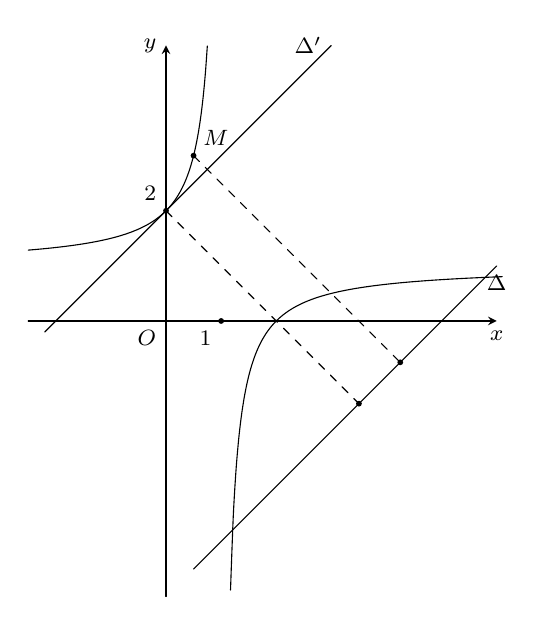
\begin{tikzpicture}[scale=0.7,font=\footnotesize,line join = round, line cap = round,>=stealth]
			\def\hsf{((\x)-2)/((\x)-1)}
			\def\hsg{1*(\x)-5}
			\def\hsh{1*(\x)+2}
			\draw[->] (-2.5,0)--(0,0)node[below left]{$O$}--(6,0)node[below]{$x$};
			\draw[->] (0,-5)--(0,5)node[left]{$y$};
			\draw[dashed,thin] (0,2)--(7/2,-3/2) (.5,3)--(17/4,-3/4);
			\draw[samples=100,domain=-2.5:.75,smooth] plot (\x, {\hsf});
			\draw[samples=100,domain=1.17:6.1,smooth] plot (\x, {\hsf});
			\draw[samples=100,domain=.5:6,smooth] plot (\x, {\hsg}) node[below]{$\Delta$};
			\draw[samples=100,domain=-2.2:3,smooth] plot (\x, {\hsh}) node[ left]{$\Delta'$};
			\fill (0,2)node[above left]{$2$} circle (1.5pt);\fill (7/2,-3/2)circle (1.5pt);\fill (.5,3)node[ above right]{$M$} circle (1.5pt);\fill (17/4,-3/4)circle (1.5pt);\fill (1,0)node[below left]{$1$} circle (1.5pt);
			\end{tikzpicture}
		\end{center}
		Gọi $\Delta'$ là tiếp tuyến của $(C)$ tại điểm $A$ có hoành độ nhỏ hơn 1 và song song với $\Delta$.\\
		Ta có hoành độ điểm $A$ là nghiệm phương trình $y'=1\Leftrightarrow\dfrac{1}{\left( x-1\right) ^2}=1\Leftrightarrow\hoac{&x=0\\&x=2}$; mà hoành độ $A$ nhỏ hơn 1 nên $x=0$ hay $A\left( 0;2\right) $.\\
		Khi đó, với mọi điểm $M \left( x_M<1\right) )$ ta đều có $d=\mathrm{d}\left( M,\Delta\right) \geq\mathrm{d}\left( A,\Delta\right) $. Dấu bằng khi tại $M\equiv A$.\\
		$d_{\min} =\mathrm{d}(A;\Delta)=\dfrac{7}{\sqrt{2}}$.}
\end{ex}
\begin{ex}%[2D1K5-6]%Câu 21.%[Trần Ngọc Phú]
	Cho hàm số $y=x^3-3x+1\left( C\right) $ và đường thẳng $d\colon y=-3x+1$. Gọi $M\left( p;q\right) $ là điểm có hoành độ dương nằm trên $d$ thỏa mãn các tiếp tuyến của $\left( C\right) $ kẻ từ $M$ vuông góc với nhau. Khi đó $p^2+q^2$ bằng 
	\choice
	{\True $\dfrac{481-108\sqrt{10}}{81}$}
	{$\dfrac{720+54\sqrt{80}}{81}$}
	{$\dfrac{720-54\sqrt{80}}{81}$}
	{$\dfrac{481+108\sqrt{10}}{81}$}
	\loigiai{
		$y=x^3-3x+1\left( C\right) $, $y'=3x^2-3$.\\
		Nhận xét $d\colon y=-3x+1$ là một tiếp tuyến của $\left( C\right) $.\\
		Từ $M(p;q)$ thuộc $d$ kẻ được tiếp tuyến vuông góc với $d$ kéo theo $M=d\cap\Delta$ trong đó $\Delta$ là tiếp tuyến của $\left( C\right) $ có hệ số góc bằng $\dfrac{1}{3}$.\\
		$y'=\dfrac{1}{3}\to 3x^2-3=\dfrac{1}{3}\Leftrightarrow x=\pm\dfrac{\sqrt{10}}{3}$. Do $M$ có hoành độ dương $x=\dfrac{\sqrt{10}}{3}$ thỏa mãn.\\
		$\Delta$: $y=\dfrac{1}{3}x-\dfrac{20\sqrt{10}}{27}+1$.\\
		Xét hệ $\heva{&y=\dfrac{1}{3}x-\dfrac{20\sqrt{10}}{27}+1\\&y=-3x+1}\Leftrightarrow\heva{&x=\dfrac{2\sqrt{10}}{9}\\&y=\dfrac{-2\sqrt{10}}{3}+1}\Rightarrow M\left(\dfrac{2\sqrt{10}}{9};1-\dfrac{2\sqrt{10}}{3}\right)$.\\
		Vậy $p^2+q^2=\dfrac{481-108\sqrt{10}}{81}$.}
\end{ex}
\begin{ex}%[2D1Y5-2]%Câu 22.%[Trần Ngọc Phú]
	Cho hàm số $y=\dfrac{x+2}{x+1}$ có đồ thị $\left( C\right)$. Số điểm có tọa độ nguyên thuộc $\left( C\right)$ là 
	\choice
	{\True $2$}
	{$5$}
	{$3$}
	{$4$}
	\loigiai{
		Ta có $y=\dfrac{x+2}{x+1}=1+\dfrac{1}{x+1}$.\\
		Gọi $M\left( x_0;y_0\right) $ có tọa độ nguyên thuộc $\left( C\right)$ nên $\heva{&x_0\in \mathbb{Z}\\&y_0=1+\dfrac{1}{x_0+1}\in \mathbb{Z}}\Leftrightarrow\hoac{&\heva{&x_0=0\\&y_0=2}\\&\heva{&x_0=-2\\&y_0=0}}$.}
\end{ex}
\begin{ex}%[2D1K5-6]%Câu 23.%[Trần Ngọc Phú]
	Cho hàm số $y=\dfrac{x+1}{x}$ có đò thị $\left( C\right)$. Hỏi trên đồ thị hàm số $\left( C\right)$ về phía phải trục tung có bao nhiêu điểm mà tại đó ta dựng được tiếp tuyến cắt hai trục tọa độ tạo thành tam giác cân. 
	\choice
	{vô số}
	{$2$}
	{\True $1$}
	{$0$}
	\loigiai{
		Ta có $y'=-\dfrac{1}{x^2}$.\\
		Giả sử $M\left( x_0;y_0\right) \in\left( C\right)$; $d$ là tiếp tuyến của đồ thị $\left( C\right)$ tại điểm $M$.\\
		Phương trình $d$ là $y=-\dfrac{1}{x_0^2}\left( x-x_0\right) +\dfrac{x_0+1}{x_0}$.\\
		Gọi $A=d\cap Ox\Rightarrow A\left(x_0^2+2x_0;0\right)$ vì $A$ nằm bên phải trục tung nên $x_0\in(-\infty;-2)\cup(0;+\infty)$.\\
		$B=d\cap Oy\Rightarrow B\left(0;\dfrac{x_0+2}{x_0}\right)$.\\
		Suy ra $OA=x_0^2+2x_0;OB=\dfrac{x_0+2}{x_0}$.\\
		Tam giác $OAB$ cân $\Leftrightarrow OA=OB\Leftrightarrow x_0^2+2x_0=\dfrac{x_0+2}{x_0}$ \\
		$ \Leftrightarrow x_0^3+2x_0^2-x_0-2=0\Leftrightarrow\hoac{&x_0=1\\&x_0=-1 \text{ (loại)}\\&x_0=-2 \text{ (loại)}.} $ \\
		Vậy tồn tại một điểm duy nhất thỏa mãn yêu cầu bài toán.}
\end{ex}
\begin{ex}%[2D1K5-2]%Câu 24.%[Trần Ngọc Phú]
	Biết đồ thị hàm số $y=(m-4)x^3-6(m-4)x^2-12mx+7m-18$ có ba điểm cố định thẳng hàng. Viết PTĐT đi qua ba điểm cố định đó. 
	\choice
	{\True $y=-48x+10$}
	{$y=\sqrt{3}x-1$}
	{$y=x-2$}
	{$y=2x-1$}
	\loigiai{
		Giả sử, $M\left( x_0;y_0\right) $ là điểm cố định mà đồ thị hàm số luôn đi qua.\\
		Khi đó $y_0=\left( m-4\right) x_0^3-6\left( m-4\right) x_0^2-12mx_0+7m-18,\forall m$ \\
		$ \Leftrightarrow\left(x_0^3-6x_0^2-12x_0+7\right)m-4x_0^3+24x_0^2-18-y_0=0,\forall m $.\\
		Suy ra, $\heva{&x_0^3-6x_0^2-12x_0+7=0\\&-4x_0^3+24x_0^2-18-y_0=0}$.\\ Do đó $-4\left( 12x_0-7\right) -18-y_0=0$ 
		$ \Leftrightarrow y_0=-48x_0+10 $.\\
		Vậy PTĐT cần tìm là $y=-48x+10$.}
\end{ex}
\begin{ex}%[2D1B5-4]%Câu 25.%[Trần Ngọc Phú]
	Hàm số $y=f\left( x\right) =x^3+ax^2+bx+c$ đạt cực tiểu tại điểm $x=1$, $f\left( 1\right) =-3$ và đồ thị hàm số cắt trục tung tại điểm có tung độ bằng $2$. Tính $T=a+b+c$. 
	\choice
	{$T=-2$}
	{\True $T=-4$}
	{$T=9$}
	{$T=1$}
	\loigiai{
		$f'\left( x\right) =3x^2+2ax+b$.\\
		Hàm số đạt cực tiểu tại điểm $x=1\Rightarrow f'\left( 1\right) =0\Rightarrow 2a+b=-3$.\\
		$f\left( 1\right) =-3\Rightarrow 1+a+b+c=-3\Rightarrow a+b+c=-4$.\\
		Đồ thị hàm số cắt trục tung tại điểm có tung độ bằng $2$ nên
		$f\left( 0\right) =2\Rightarrow c=2$.\\
		Ta có $\heva{&2a+b=-3\\&a+b+c=-4\\&c=2}\Rightarrow\heva{&a=3\\&b=-9\\&c=2.}$ \\
		Khi đó $f\left( x\right) =x^3+3x^2-9x+2$; $f'(x)=3x^2+6x-9$.\\
		Ta có $f'(1)=0$ $\Rightarrow x=1$ là điểm cực tiểu.\\
		Vậy $T=a+b+c=-4$.}
\end{ex}
\begin{ex}%[2D1B5-2]%Câu 26.%[Trần Ngọc Phú]
	Cho hàm số $y=\dfrac{1-3x}{3-x}$ có đồ thị là $\left( C\right)$. Điểm $M$ nằm trên đồ thị $\left( C\right)$ sao cho khoảng cách từ $M$ đến tiệm cận đứng gấp hai lần khoảng cách từ $M$ đến tiệm cận ngang của $\left( C\right)$. Khoảng cách từ $M$ đến tâm đối xứng của $\left( C\right)$ bằng
	\choice
	{$3\sqrt{2}$}
	{\True $2\sqrt{5}$}
	{$4$}
	{$5$}
	\loigiai{
		- Gọi $M\left(m;\dfrac{1-3m}{3-m}\right)\in\left( C\right)$, với $m\neq 3$.\\
		- Đồ thị $\left( C\right)$ có đường tiệm cận đứng là $a\colon x-3=0$; tiệm cận ngang là $b\colon y-3=0$.\\
		Ta có: $\mathrm{d}(M;a)=2\cdot\mathrm{d}\left( M;b\right) \Leftrightarrow|m-3|=2\cdot\left|\dfrac{1-3m}{3-m}-3\right|$ \\
		$ \Leftrightarrow|m-3|=\dfrac{16}{|m-3|}\Leftrightarrow\hoac{&m-3=4\\&m-3=-4}\Leftrightarrow\hoac{&m=7\\&m=-1}\Rightarrow\hoac{&M_1=\left( 7;5\right) \\&M_2=\left( -1;1\right) .} $ \\
		- Đồ thị $\left( C\right)$ có tâm đối xứng là $I\left( 3;3\right) \Rightarrow IM_1=IM_2=2\sqrt{5}$.}
\end{ex}
\begin{ex}%[2D1K5-2]%Câu 27.%[Trần Ngọc Phú]
	Điểm $M\left( a; b\right) $ thuộc đồ thị hàm số $\left( C\right)\colon y=\dfrac{x-1}{x+1}$ sao cho tổng khoảng cách từ điểm $M$ đến hai trục toạ độ là nhỏ nhất. Tính $a+2b$. 
	\choice
	{$-1+\sqrt{2}$}
	{$0$}
	{\True $1-\sqrt{2}$}
	{$1-2\sqrt{2}$}
	\loigiai{
		\begin{center}
			\begin{tikzpicture}[scale=0.7,font=\footnotesize,line join = round, line cap = round,>=stealth]
			\def\hsf{((\x)-1)/((\x)+1)}
			\draw[->] (-3.5,0)--(0,0)node[below left]{$O$}--(4.5,0)node[below]{$x$};
			\draw[->] (0,-5)--(0,5)node[left]{$y$};
			\draw[dashed,thin] (-3.5,1)--(4.5,1) (-1,-5)--(-1,5); 
			\draw[] (0,0)--(0.5,-1/3);
			\draw[samples=100,domain=-.65:4.25,smooth] plot (\x, {\hsf});
			\draw[samples=100,domain=-3.5:-1.5,smooth] plot (\x, {\hsf});
			\fill (0,1)node[left]{$1$} circle (1.5pt);\fill (1,0)node[below]{$1$} circle (1.5pt);\fill (2,0)node[below]{$2$} circle (1.5pt);\fill (-2,0)node[below]{$-2$} circle (1.5pt);\fill (0,2)node[ left]{$2$} circle (1.5pt);\fill (0.5,-1/3)node[below]{$M$} circle (1.5pt);
			\end{tikzpicture}
		\end{center}
		Ta có $M\left( a; b\right) $ thuộc $\left( C\right) y=\dfrac{x-1}{x+1}\Rightarrow M\left(a;\dfrac{a-1}{a+1}\right)$.\\
		Nhận xét tổng khoảng cách từ điểm $M$ đến hai trục toạ độ nhỏ nhất khi $OM_{\min}$.\\
		Theo đồ thị $\heva{&x_M\in\left( 0; 1\right) \\&y_M\in\left( -1; 0\right) }\Rightarrow\heva{&a>0\\&\dfrac{a-1}{a+1}<0.}$ \\
		Tổng khoảng cách $d=|a|+\left|\dfrac{a-1}{a+1}\right|=a+\dfrac{1-a}{a+1}=a+\dfrac{2}{a+1}-1=a+1+\dfrac{2}{a+1}-2\geq 2\sqrt{2}-2$. \\
		$ \Rightarrow d_{\min}\Leftrightarrow a+1=\dfrac{2}{a+1}\Leftrightarrow\hoac{&a=-1+\sqrt{2}>0\\&a=-1-\sqrt{2}<0.} $ \\
		Vậy $M\left(-1+\sqrt{2}; 1-\sqrt{2}\right)\Rightarrow\heva{&a=-1+\sqrt{2}\\&b=1-\sqrt{2}}\Rightarrow a+2b=1-\sqrt{2}$.}
\end{ex}
\begin{ex}%[2D1G5-6]%Câu 28.%[Trần Ngọc Phú]
	Cho hàm số $y=\left| x\right|  ^3-3x^2+1 \left( C\right) $. Hỏi trên trục $Oy$ có bao nhiêu điểm $A$ mà qua $A$ có thể kẻ đến $(C)$ đúng ba tiếp tuyến?
	\choice
	{$3$}
	{\True $1$}
	{$0$}
	{$2$}
	\loigiai{
		\textbf{Cách 1:} Sử dụng đồ thị hàm số.\\
		$\bullet$ Vẽ đồ thị hàm số $y=x^3-3x^2+1$ có đồ thị $\left( C\right)$. 
		\begin{center}
			\begin{tikzpicture}[scale=0.7,font=\footnotesize,line join = round, line cap = round,>=stealth]
			\def\hsf{1*(\x)^3-3*(\x)^2+1}
			\draw[->] (-2.5,0)--(0,0)node[below left]{$O$}--(4.5,0)node[below]{$x$};
			\draw[->] (0,-4)--(0,4)node[left]{$y$};
			%\draw[dashed,thin] (1,0)--(1,3)--(0,3) (0,1)--(2,1)--(2,0) (0,5)--(3,5)--(3,0);
			\draw[samples=100,domain=-1.05:3.25,smooth] plot (\x, {\hsf});
			\fill (0,1)node[left]{$1$} circle (1.5pt);\fill (1,0)node[below]{$1$} circle (1.5pt);\fill (2,0)node[below]{$2$} circle (1.5pt);\fill (-2,0)node[below]{$-2$} circle (1.5pt);\fill (0,2)node[ left]{$2$} circle (1.5pt);
			\end{tikzpicture}
		\end{center}
		$\bullet$ Hàm số $y=\left| x\right| ^3-3x^2+1=\heva{&x^3-3x^2+1\text{ khi }x\geq 0\\&-x^3-3x^2+1 \text{ khi }x<0}$ có đồ thị $\left( C'\right)$ bằng cách\\
		+ Giữ nguyên phần đồ thị $\left( C\right)$ nằm bên phải trục $(0;1)$ và bỏ phần $\left( C\right)$ nằm bên trái $Oy$.\\
		+ Lấy đối xứng phần đồ thị $\left( C\right)$ nằm bên phải trục $Oy$ qua $Oy$. 
		\begin{center}
			\begin{tikzpicture}[scale=0.7,font=\footnotesize,line join = round, line cap = round,>=stealth]
			\def\hsf{1*(\x)^3-3*(\x)^2+1}
			\def\hsg{-1*(\x)^3-3*(\x)^2+1}
			\draw[->] (-3.5,0)--(0,0)node[below left]{$O$}--(4.5,0)node[below]{$x$};
			\draw[->] (0,-4)--(0,4)node[left]{$y$};
			\draw[samples=100,domain=0:3.25,smooth] plot (\x, {\hsf});
			\draw[samples=100,domain=-3.25:0,smooth] plot (\x, {\hsg});
			\fill (0,1)node[left]{$1$} circle (1.5pt);\fill (1,0)node[below]{$1$} circle (1.5pt);\fill (2,0)node[below]{$2$} circle (1.5pt);\fill (-2,0)node[below]{$-2$} circle (1.5pt);\fill (0,2)node[ left]{$2$} circle (1.5pt);
			\end{tikzpicture}
		\end{center}
		$\bullet$ Hàm $y=\left| x\right| ^3-3x^2+1$ có đồ thị hàm chẵn nên đối xứng qua $Oy$. Do vậy nếu từ điểm $A$ thuộc $Oy$ kẻ được tới nửa đồ thị bên phải bao nhiêu tiếp tuyến thì kẻ qua đồ thị bên trái bấy nhiêu tiếp tuyến. Suy ra để kẻ được số lẻ tiếp tuyến thì chỉ xảy ra ở điểm cực đại. Vậy có duy nhất điểm thỏa yêu cầu bài toán đó là $A\left( 0;1\right) $. 
		\begin{center}
			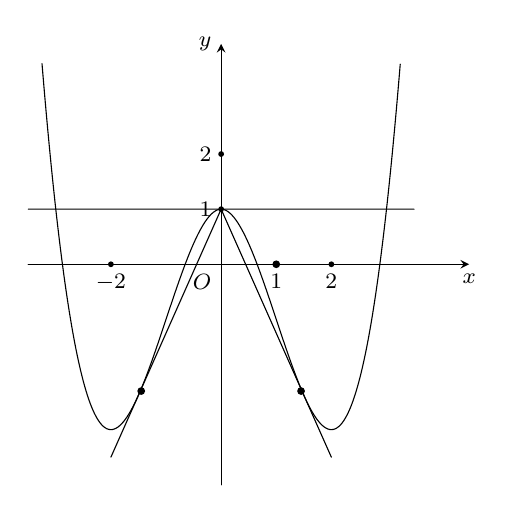
\begin{tikzpicture}[scale=0.7,font=\footnotesize,line join = round, line cap = round,>=stealth]
			\def\hsf{1*(\x)^3-3*(\x)^2+1}
			\def\hsg{-1*(\x)^3-3*(\x)^2+1}
			\draw[->] (-3.5,0)--(0,0)node[below left]{$O$}--(4.5,0)node[below]{$x$};
			\draw[->] (0,-4)--(0,4)node[left]{$y$};
			\draw[] (-3.5,1)--(3.5,1) (-2,-3.5)--(0,1)--(2,-3.5);
			\draw[samples=100,domain=0:3.25,smooth] plot (\x, {\hsf});
			\draw[samples=100,domain=-3.25:0,smooth] plot (\x, {\hsg});
			\fill (0,1)node[left]{$1$} circle (1.5pt);\fill (1,0)node[below]{$1$} circle (2pt);\fill (2,0)node[below]{$2$} circle (1.5pt);\fill (-2,0)node[below]{$-2$} circle (1.5pt);\fill (0,2)node[ left]{$2$} circle (1.5pt);\fill (-1.45,-2.3) circle (2pt);\fill (1.45,-2.3) circle (2pt);
			\end{tikzpicture}
		\end{center}
		Thử lại thấy thỏa mãn.\\
	\textbf{Cách 2.}
		Gọi tiếp tuyến với hệ số góc $k$ đi qua $A\left( 0;m\right) $ có dạng $y=kx+m;\left( d\right) $.\\
		Đường thẳng $d$ là tiếp tuyến của $\left( C\right)$ khi hệ sau có nghiệm.\\
		$\heva{&y'=f'(x)=k\\&|x|^3-3x^2+1=kx+m}(I)$.\\
		\textbf{Trường hợp 1:} nếu $x\geq 0$ thì hệ trên trở thành:\\
		$\heva{&3x^2-6x=k\\&x^3-3x^2+1=kx+m}\Rightarrow g(x)=-2x^3+3x^2+1=m$.\\
		\textbf{Trường hợp 2:} nếu $x<0$ thì hệ trên trở thành:\\
		$\heva{&-3x^2-6x=k\\&-x^3-3x^2+1=kx+m}\Rightarrow h(x)=2x^3+3x^2+1=m$.\\
		Bảng biến thiên hai hàm: $g(x); h(x)$: 
		\begin{center}
			\begin{tikzpicture}
			\tkzTabInit[nocadre=false,lgt=1.2,espcl=2.5,deltacl=0.6]
			{$x$/.6,$g'(x)$/.6,$h'(x)$/.6,ĐT/2}
			{$-\infty$ , $-1$ , $0$ , $1$ , $+\infty$}
			\tkzTabLine{ , h ,  , h , z , + , $0$ , - , }
			\tkzTabLine{ , + , $0$ , - , d , h , , h , }
			\tkzTabVar{-/$-\infty$ , +/$2$, -/$1$ , +/$2$ , -/$-\infty$}
			\end{tikzpicture}
		\end{center}
		Hệ $(I)$ có đúng 3 nghiệm khi $m=1$.\\ Vậy điểm $A\left( 0;1\right) $.}
\end{ex}
\begin{ex}%[2D1G5-3]%Câu 29.%[Trần Ngọc Phú]
	Cho hàm số $y=mx^3+x^2+\left( 1-4m\right) x-6$ có đồ thị $\left( C_m\right) $. Gọi giao điểm của đồ thị $\left( C_m\right) $ với các trục tọa độ $Ox$, $Oy$ lần lượt là $A$, $B$. Gọi $C$ là điểm thuộc $\left( C_m\right) $ sao cho diện tích tam giác $ABC$ không đổi với mọi giá trị của $m$. Khi đó diện tích tam giác $ABC$ bằng
	\choice
	{$10$}
	{\True $8$}
	{$9$}
	{$7$}
	\loigiai{
		Ta thấy $\left( C_m\right) $ đi qua các điểm cố định là $A\left( 2;0\right) $, $B\left( 0;-6\right) $ và $C\left( -2;-4\right) $.\\
		Phương trình $\left( AB\right) \colon\dfrac{x}{2}+\dfrac{y}{-6}=1\Leftrightarrow-6x+2y+12=0$.\\
		$\mathrm{d}\left( C;AB\right) =\dfrac{16}{\sqrt{40}}$. Suy ra $S_{ABC}=\dfrac{1}{2}AB\cdot\mathrm{d}\left( C;AB\right) =8$.}
\end{ex}
\begin{ex}%[2D1G5-2]%Câu 30.%[Trần Ngọc Phú]
	Gọi $M\left( a;b\right) $ là điểm thuộc đồ thị hàm số $y=\dfrac{2x+1}{x+2}$ có khoảng cách từ $M$ đến đường thẳng $d\colon y=3x+6$ nhỏ nhất. Tìm giá trị của biểu thức $T=3a^2+b^2$. 
	\choice
	{\True $T=4$}
	{$T=3$}
	{$T=9$}
	{$T=10$}
	\loigiai{
		$M\left( a;b\right) $ là điểm thuộc đồ thị hàm số $y=\dfrac{2x+1}{x+2}\Rightarrow\heva{&a\neq-2\\&b=\dfrac{2a+1}{a+2}=2-\dfrac{3}{a+2}.}$ \\
		$d\colon y=3x+6$ hay $d\colon 3x-y+6=0$.\\
		$\mathrm{d}\left( M,d\right) =\dfrac{\left|3a-2+\dfrac{3}{a+2}+6\right|}{\sqrt{10}} =\dfrac{\left|3\left( a+2\right) +\dfrac{3}{a+2}-2\right|}{\sqrt{10}}$.\\
		Nếu $a >-2\Rightarrow\left( a+2\right) +\dfrac{1}{a+2}\geq 2\Rightarrow 3\left( a+2\right) +\dfrac{3}{a+2}-2\geq 4>0\Rightarrow\mathrm{d}\left( M,d\right) \geq\dfrac{4}{\sqrt{10}}$.\\
		Nếu $a <-2\Rightarrow-\left( a+2\right) +\dfrac{1}{-\left( a+2\right) }\geq 2\Rightarrow\left( a+2\right) +\dfrac{1}{a+2}\leq-2\Rightarrow 3\left( a+2\right) +\dfrac{3}{a+2}-2\leq-8<0$. \\
		$ \Rightarrow\mathrm{d}\left( M,d\right) \geq\dfrac{8}{\sqrt{10}} $.\\
		Do đó $\min\mathrm{d}\left( M,d\right) =\dfrac{4}{\sqrt{10}}\Leftrightarrow a+2=1\Leftrightarrow a=-1\Rightarrow b=-1\Rightarrow T=3a^2+b^2=4$.}
\end{ex}
\Closesolutionfile{ans}	

